\section{离散傅里叶变换的性质}

本节介绍DFT的性质。
由于DFT的定义域受限,所以在做坐标平移时和DTFT不同。

本节要点:
\begin{itemize}
    \item 理解循环平移(时移和频移);
    \item 掌握循环卷积。
\end{itemize}

%============================================================
\subsection{循环时移和循环频移}

\begin{definition}[循环时移]
假设离散信号$x\left[ n \right] ,n\in \left[ 0,N \right) $,当有$q\in \mathbb{Z} $,$x\left[ n-q \right] $的超出定义域部分值挪到另一边,这样的时移称为{\bf 循环时移},记为$x\left[ n-q,\mathrm{mod}N \right] $,即:
\[
x\left[ n-q,\mathrm{mod}N \right] =\begin{cases}
	x\left[ N-q \right]&		n=0\\
	x\left[ N-q+1 \right]&		n=1\\
	\vdots&		\\
	x\left[ N-1 \right]&		n=q-1\\
	x\left[ 0 \right]&		n=q\\
	x\left[ 1 \right]&		n=q+1\\
	\vdots&		\\
	x\left[ N-q-1 \right]&		n=N-1\\
\end{cases}
\]
\end{definition}

离散信号的循环时移可以用圆助记,信号$x\left[ n \right] ,n\in \left[ 0,N \right) $可以认为是$N$个以逆时针方向平均分布在一单位圆上的点集,可取正下方为$x\left[ 0 \right] $。
$x\left[ n-q,\mathrm{mod}N \right] ,q>0$为将圆逆时针转$q$格。
例如$x\left[ n-3,\mathrm{mod}8 \right] $:
\begin{figure}[h]
\centering
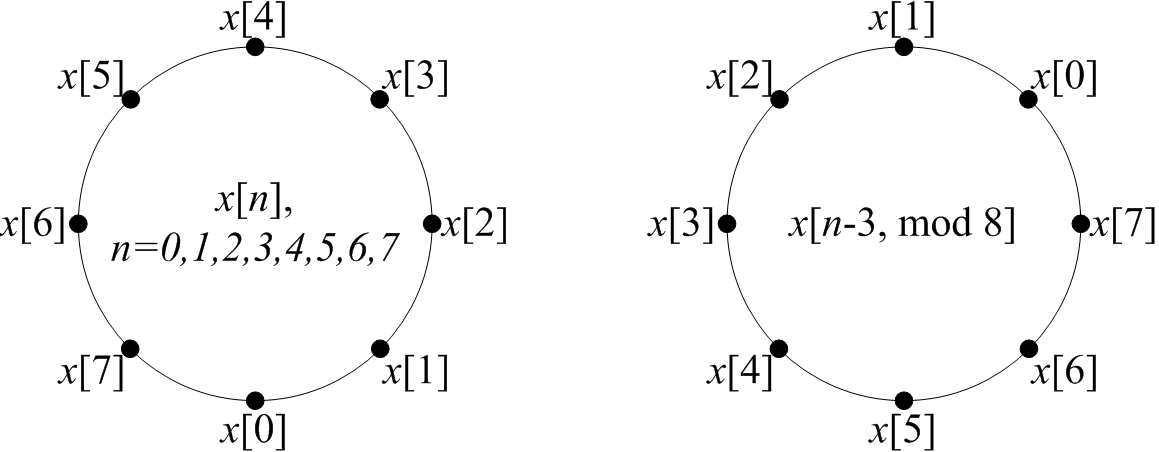
\includegraphics[height=4cm]{6.4.1-1.png}
\end{figure}

同样可以定义{\bf 循环频移}$X\left[ m-q,\mathrm{mod}N \right] $,略。

%============================================================
\subsection{循环卷积}

之前定义了离散函数的卷积:
\[
a\left[ n \right] \ast b\left[ n \right] =\sum_{i=-\infty}^{+\infty}{a\left[ i \right] b\left[ n-i \right]}
\]
由于DFT中信号只在$\left[ 0,N \right) $上有定义,所以可以仿照循环时移的定义,定义一个循环的卷积。

\begin{definition}[循环卷积]
对于两个离散函数$a\left[ n \right] ,b\left[ n \right] ,n\in \left[ 0,N \right) $,我们称和式$\sum_{i=0}^{N-1}{a\left[ i \right] b\left[ n-i,\mathrm{mod}N \right]}$为$a\left[ n \right] ,b\left[ n \right] $的{\bf 循环卷积}(circular convolution),记为$a\left[ n \right] \circledast b\left[ n \right] $,即:
\[
a\left[ n \right] \circledast b\left[ n \right] =\sum_{i=0}^{N-1}{a\left[ i \right] b\left[ n-i,\mathrm{mod}N \right]}
\]
为表区分,特别将前者称为{\bf 线性卷积}(linear convolution)。
\end{definition}

\begin{theorem}[卷积相等定理]
若有两个离散函数$a\left[ n \right] ,b\left[ n \right] ,n\in \left[ 0,N \right) $,如果将其零项扩充至$2N-2$,即:
\[
a\left[ n \right] =b\left[ n \right] =0 \qquad n\in \left[ N,2N-1 \right)
\]
则离散函数$a\left[ n \right] =b\left[ n \right] =0,n\in \left[ N,2N-1 \right) $的线性卷积和循环卷积结果一致,即:
\[
a\left[ n \right] \ast b\left[ n \right] =a\left[ n \right] \circledast b\left[ n \right]
\]
\end{theorem}

所以通常来讲,DFT和DTFT结果是不一致的,除非对信号进行零扩充。

%============================================================
\subsection{DFT的性质}

{\bf 线性性}
\[
ax\left[ n \right] +by\left[ n \right] \leftrightarrow aX\left[ m \right] +bY\left[ m \right]
\]

{\bf 时移性、频移性}
\begin{align*}
&x\left[ n-q,\mathrm{mod}N \right] \leftrightarrow X\left[ m \right] e^{-i\frac{2\pi mq}{N}} \\
&e^{i\frac{2\pi mq}{N}}x\left[ n \right] \leftrightarrow X\left[ m-q,\mathrm{mod}N \right]
\end{align*}

{\bf 反转性}
\[
x\left[ -n,\mathrm{mod}N \right] \leftrightarrow X\left[ -m,\mathrm{mod}N \right]
\]

{\bf 卷积}
\begin{align*}
&x\left[ n \right] \circledast y\left[ n \right] \leftrightarrow X\left[ m \right] Y\left[ m \right] \\
&x\left[ n \right] y\left[ n \right] \leftrightarrow \frac{1}{N}X\left[ m \right] \circledast Y\left[ m \right]
\end{align*}

{\bf Parseval定理}
\[
\sum_{n=0}^{N-1}{x\left[ n \right] y\left[ n \right]}=\frac{1}{N}\sum_{m=0}^{N-1}{\bar{X}\left[ m \right] Y\left[ m \right]}
\]




